%!TEX program = xelatex
% 完整编译: xelatex -> bibtex -> xelatex -> xelatex
\documentclass[lang=cn,11pt,a4paper]{elegantpaper}
\lstset{style=bash}

\title{定位与导航实验报告}
\author{Wugang Meng \\ Xiang Feng}
\institute{哈尔滨工业大学(威海)}

\version{0.1}
\date{\zhtoday}

\begin{document}

\maketitle

\begin{abstract}
本文介绍了《**智能感知系统》项目中的定位与建图实验、自主导航实验的理论基础、详尽的软件执行流程和具体参数。
为了本次实验的可复现性,除提供程序源码外还详述了本次实验的测试大纲。包括但不限于本次实验的测试环境,软件硬件条件以及实验的具体步骤和已达到的实验指标,并体现了实验结果的有效性。
\keywords{定位与建图,自主导航,试验大纲}
\end{abstract}


\section{定位与导航系统程序设计与实现}

\subsection{自适应蒙特卡洛定位系统}

\begin{figure}[htbp]
  \centering
  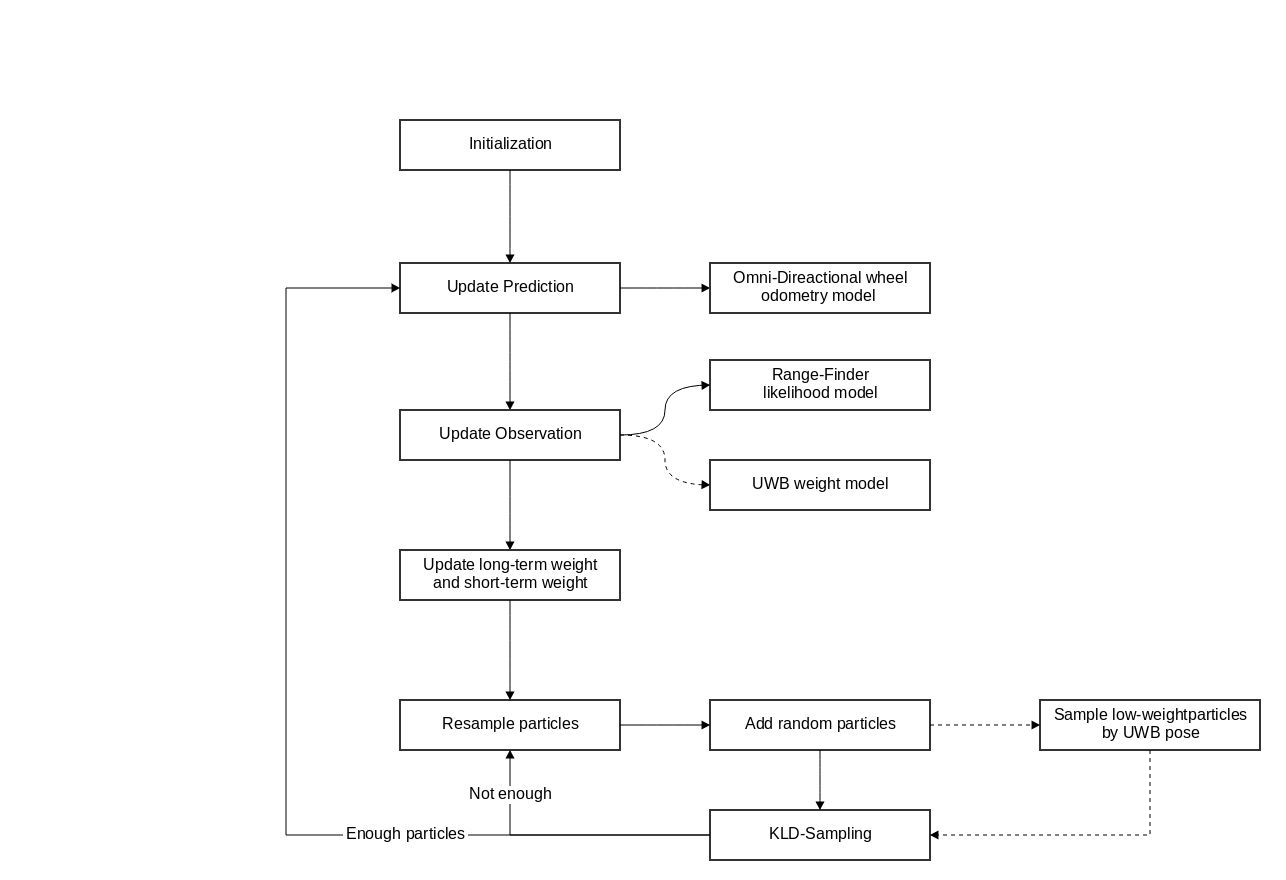
\includegraphics[width=\textwidth]{amcl.png}
  \caption{自适应蒙特卡洛定位算法流图}
  \label{fig:amcl}
\end{figure}

自适应蒙特卡洛定位( AMCL, Adaptive Monte Carlo Localization)是一套适用于二维机器人运动的定位算法。
其主要的算法原理源于算法\ref{MCL}, 算法\ref{Augmented_MCL}, 和算法\ref{KLD_MCL}算法的结合与实现。
Motion Model和Sensor Model,用于AMCL中运动的预测和粒子权重的更新。
本课题内部集成的AMCL,功能上添加了随机角度、随机位置和角度的初始化支持,以便于竞技比赛中的快速部署。
\begin{algorithm}
  \caption{蒙特卡洛定位算法}
  \label{MCL}
  \KwIn{$\mathcal X_{t-1}$,$ u_t$,$ z_t$,$ m$}
  \KwOut{$\mathcal X_{t}$}
  $\bar{\mathcal X_t} = \mathcal X_t = \emptyset$ \\
  \For{$m=1$ $\mathbf{to}$ $M$}
  {
      $sample\,{ x_t}^{[m]} \sim p( x_t|u_t,{ x_{t-1}^{[m]}}, m)$ \\
      ${ w_t}^{[m]}=p( z_t|{ x_t}^{[m]}, m)$ \\
      $\bar{\mathcal X_t} = \bar{\mathcal X_t} + \langle { x_t}^{[m]},{ w_t}^{[m]} \rangle$
  }
  \For{$m=1$ ${to}$ $M$}
  {
      $\mathbf{draw}\, i\, \mathbf{with}\,\mathbf{probability}\,\propto  {w_t}^{[i]}$ \\
      $\mathbf{add}\,{ x_t}^{[i]}\,\mathbf{to}\,\mathcal X_{t}$
  }
\end{algorithm}

\begin{algorithm}
  \caption{增强蒙特卡洛定位算法}
  \label{Augmented_MCL}
  \KwIn{$\mathcal X_{t-1}$,$ u_t$,$ z_t$,$ m$}
  \KwOut{$\mathcal X_{t}$}
  $\mathbf{static}\, w_{slow}\, w_{fast}$\\
  $\bar{\mathcal X_t} = \mathcal X_t = \emptyset$ \\
  \For{$m=1$ $\mathbf{to}$ $M$}
  {
      $sample\,{ x_t}^{[m]} \sim p( x_t|u_t,{ x_{t-1}^{[m]}}, m)$ \\
      ${ w_t}^{[m]}=p( z_t|{ x_t}^{[m]}, m)$ \\
      $\bar{\mathcal X_t} = \bar{\mathcal X_t} + \langle { x_t}^{[m]},{ w_t}^{[m]} \rangle$\\
      $w_{avg} += \frac{1}{M} { w_t}^{[m]}$
  }
  $w_{slow}+=\alpha_{slow}(w_{avg}-w_{slow})$ \\
  $w_{fast}+=\alpha_{fast}(w_{avg}-w_{fast})$ \\
  \For{$m=1$ ${to}$ $M$}
  {
      $\mathbf{draw}\, i\, \mathbf{with}\,\mathbf{probability}\,\propto  {w_t}^{[i]}$ \\
      $\mathbf{add}\,{ x_t}^{[i]}\,\mathbf{to}\,\mathcal X_{t}$
  }
\end{algorithm}

\begin{algorithm}
  \caption{库尔贝科-莱布勒散度采样蒙特卡洛定位算法}
  \label{KLD_MCL}
  \KwIn{$\mathcal X_{t-1}$,$ u_t$,$ z_t$,$ m$, $\varepsilon$, $\delta $}
  \KwOut{$\mathcal X_{t}$}
  $X_t = \emptyset$ \\
  $M=0$,$M_{\chi }=0$,$k=0$\\
  \For{$\mathbf{all}$ $b$ $\mathbf{in}$ $H$}
  {
    $b = \mathbf{empty}$
  }
  \While{$M < M_{\chi} \Vert M < M_{\chi min}  $}
  {
    $\mathbf{draw}\, i\, \mathbf{with}\,\mathbf{probability}\,\propto  {w_t}^{[i]}$ \\
    ${x_t}^{[m]} = \mathbf{smaple\_Motion\_model}(u_t,x_{t-1}^{[m]})$ \\
    ${w_t}^{[m]} = \mathbf{measurement\_model}(z_t,x_{t}^{[m]},m)$ \\
    $X_t += \left\langle {x_t}^{[m]},{w_t}^{[m]}\right\rangle $ \\
    \If{${x_t}^{[m]}$ $\mathbf{falls}$ $\mathbf{in}$ $\mathbf{empty}$ $\mathbf{bin}$ $b$}
    {
      $k+=1$\\
      $b = \mathbf{non-empty}$\\
      \If{$k > 1$}
      {
        $M_{\chi} \coloneqq \frac{k-1}{2\varepsilon } \{ 1- \frac{2}{9(k-1)} + \sqrt{\frac{2}{9(k-1)}} z_{1-\delta }\} $
      }
    }
    $M += 1$
  }
\end{algorithm}

AMCL算法的设计详细参数如所表\ref{tab:amcl}所示:
\begin{table}[!htbp]
  \centering
  \caption{AMCL设计参数}\label{tab:amcl}
  \begin{tabular}{cc}
    \toprule
    参数名称  & 参考数值  \\
    \midrule
    粒子滤波器的最小粒子数  & 50                \\
    粒子滤波器的最大粒子数  & 200               \\
    滤波器更新的位移阈值   & 0.1               \\
    滤波器更新的旋转阈值   & 0.5               \\
    机器人运动模型      & 全向轮模型 \\
    里程计模型的误差参数   & 0.05              \\
    雷达的最小有效测距距离  & 0.15m             \\
    雷达的最大有效测距距离  & 8m                \\
    雷达的波束        & 90$^{\circ}$              \\
    忽略波束的障碍物距离阈值 & 20cm              \\
    重采样周期        & 不重采样             \\
    $\alpha_{slow}$ & 0.001\\
    $\alpha_{fast}$ & 0.1\\
    $\varepsilon $  & 0.05\\
    $1-\delta  $  & 0.99\\
  \bottomrule
  \end{tabular}%
\end{table}%

\subsection{全局路径规划系统}

全局路径规划(简称全局规划)是导航系统中运动规划的第一个步骤,在给定目标位置后,根据感知的全局代价地图搜索得到一条无碰撞的最短路径(即一系列离散的坐标点),
然后作为输入传递给局部轨迹规划模块控制机器人的具体运动。
核心规划节点的执行流程如下:
\begin{enumerate}
  \item 初始化Actionlib Server,构建可视化的publisher。
  \item 读取参数。
  \item 创建tf listener,global\_costmap对象。
  \item 创建具体算法的planner对象。
  \item 回调队列在主线程开始回调,同时线程Actionlib Server Callback也开始回调。
\end{enumerate}
规划线程执行流程和Actionlib Server Callback线程执行流程如图\ref{fig:gp}和图\ref{fig:acb}所示。
\begin{figure}[htbp]
  \centering
  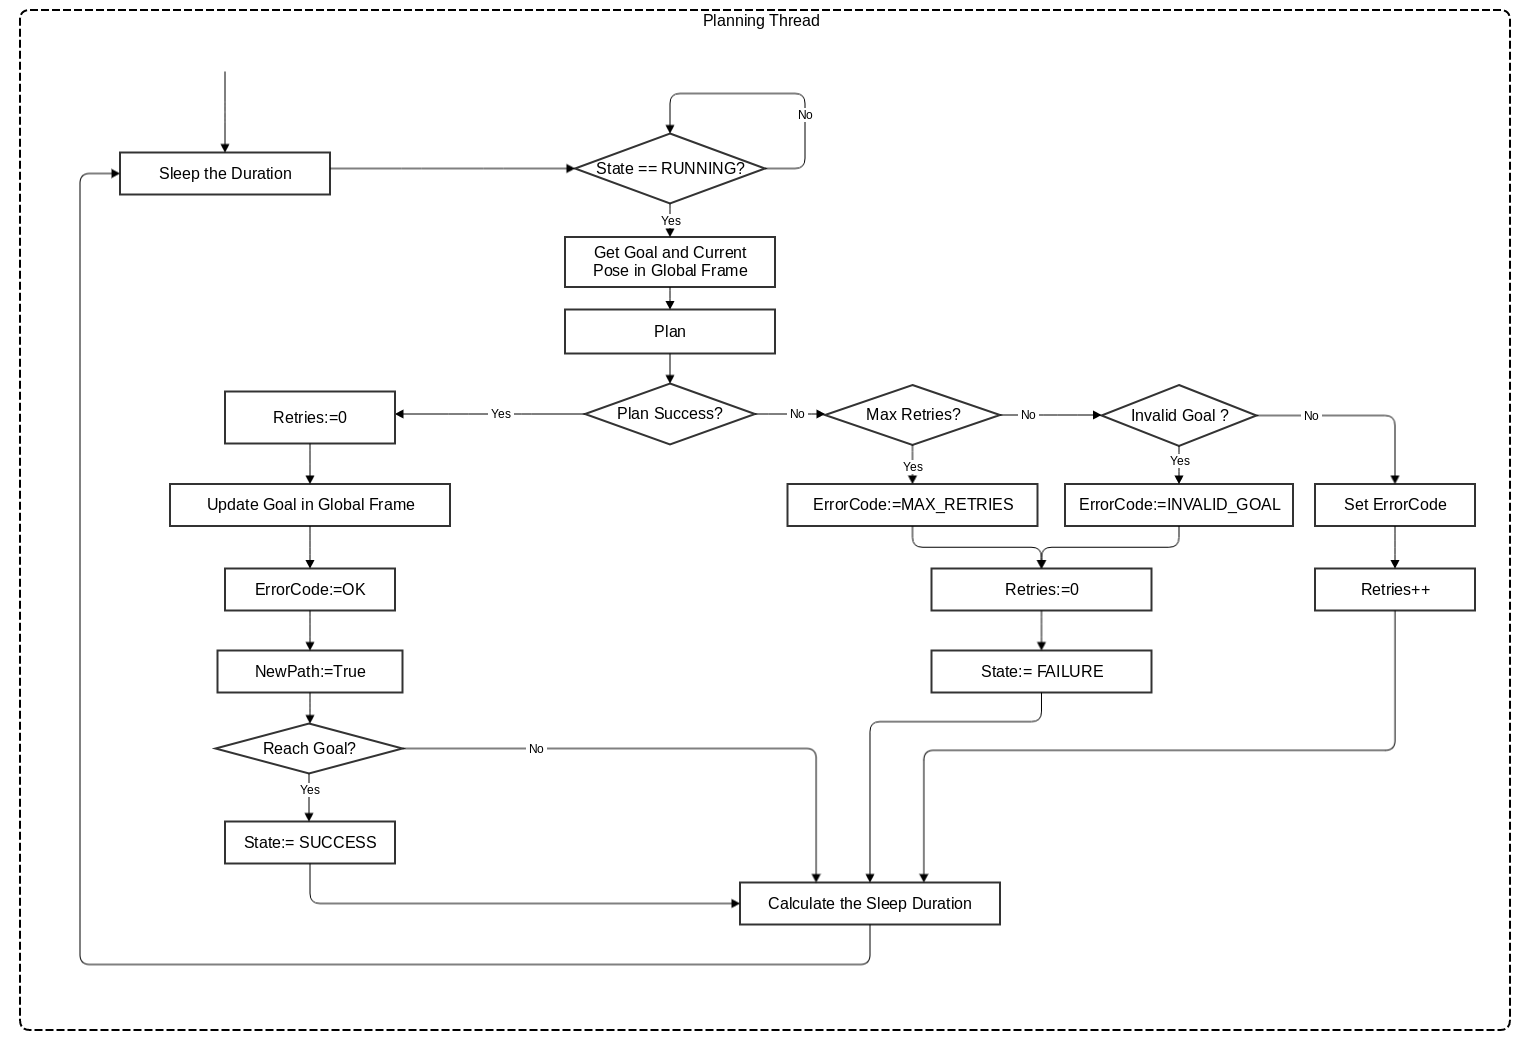
\includegraphics[width=\textwidth]{gp.png}
  \caption{全局规划线程执行流程}
  \label{fig:gp}
\end{figure}
\begin{figure}[htbp]
  \centering
  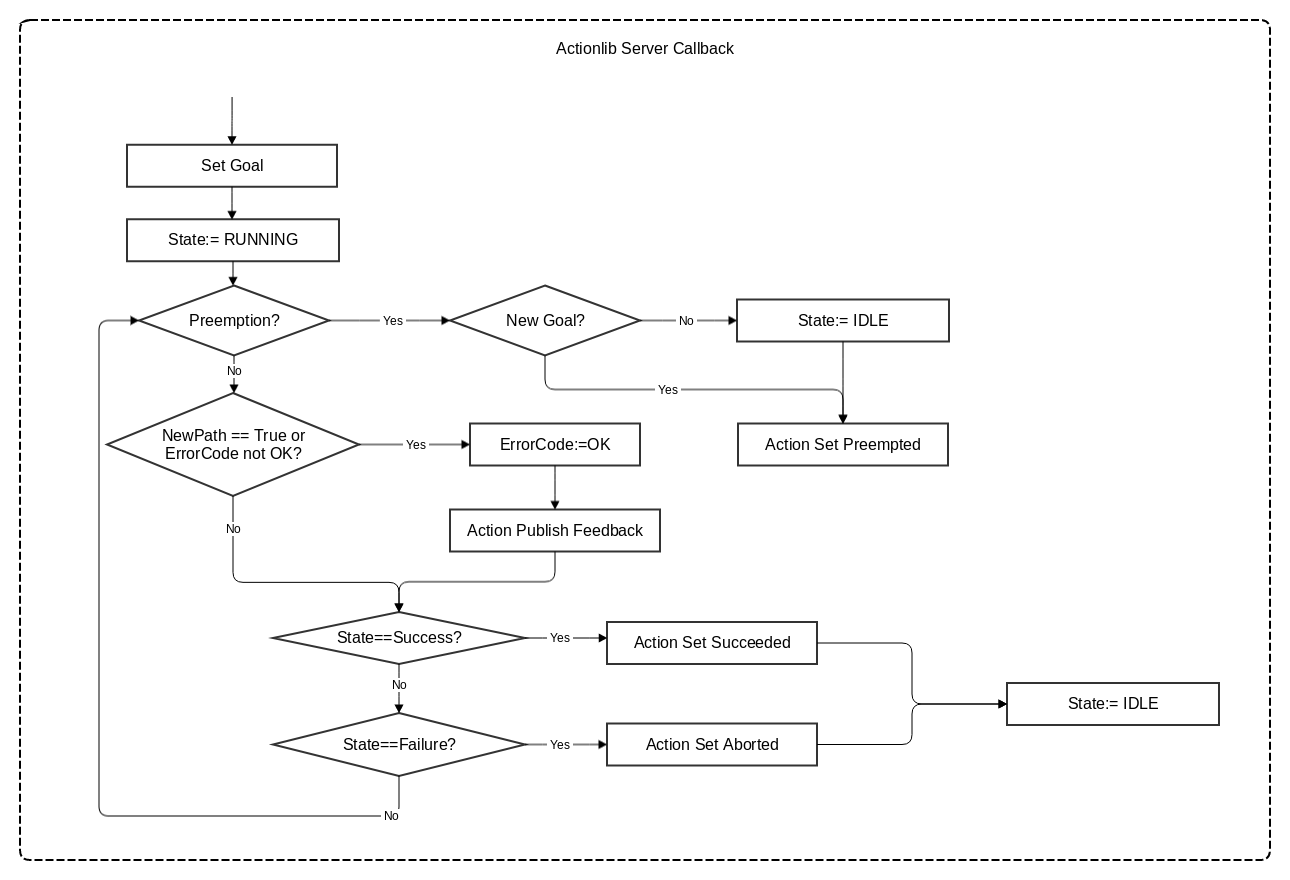
\includegraphics[width=\textwidth]{acb.png}
  \caption{Actionlib Server Callback线程执行流程}
  \label{fig:acb}
\end{figure}


\section{测试概要}

\subsection{测试目标}
进行本实验的目的是验证毫米波传感器能否与机器人操作系统(ROS)环境中流行的地图和导航库一起使用,这是许多机器人技术人员所熟悉的。
本实验将Octomap服务器和move\_base库与TI的mmWave ROS驱动程序软件包以及DJI RoboMaster底盘库一起使用,以与TI mmWave传感器接口。本实验支持使用IWR1443ISK ES1.0 EVM或IWR1443ISK ES2.0 EVM。借助TI驱动程序和\href{ros.org}{ROS社区}的软件,工程师可以快速,轻松地评估机器人导航和避开物体。
本实验室采用四个传感器一起使用。通过使用四个传感器,该机器人可以具有$360^{\circ}$视野,因此该机器人能够检测周围的物体,以便更好地进行地图绘制和导航。

\subsection{测试环境}
\subsubsection{场地环境}
本实验采用DJI RMUC 的核心比赛场地,也被称为“战场”。如图所示\ref{fig:map}战场是一个长为 28 米、宽为 15 米的区域,内部为木质结构,表
面贴地胶(厚度 3mm),主要包含基地区、高地区、资源岛区、补给区和飞行区等。战场外围有上边沿距离战场地面高度为 2.4 米的黑色钢制围挡。
全文描述的所有场地道具的尺寸误差均在$±5\%$以内。场地说明图纸尺寸参数单位为mm。

\begin{figure}[htbp]
  \centering
  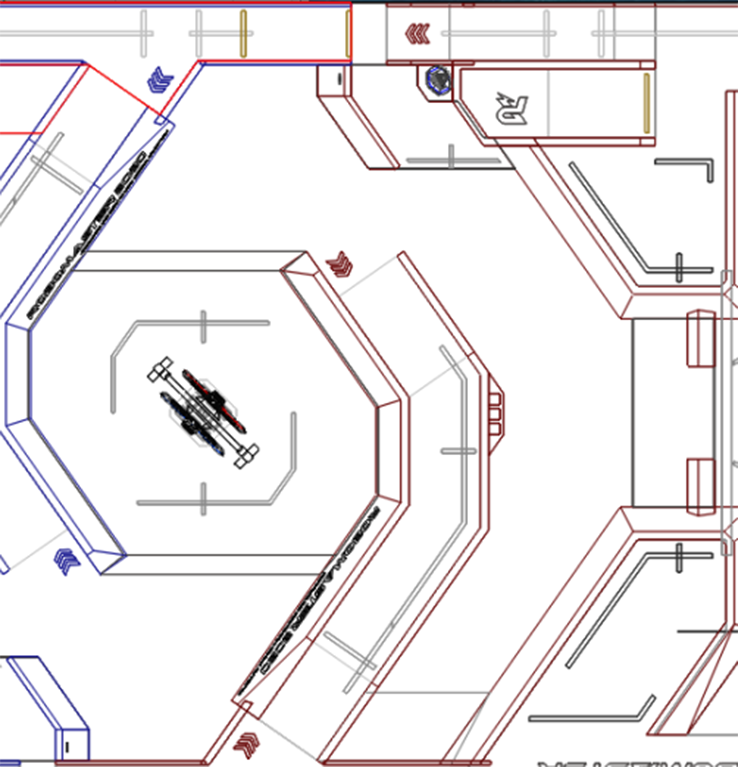
\includegraphics[width=\textwidth]{map.png}
  \caption{测试场地渲染图}
  \label{fig:map}
\end{figure}

\subsubsection{硬件设备}
移动作战平台基于模块化设计,分为动力模块,感知模块,控制模块和计算模块。所有模块支持快拆结构,各模块可单独编程与调试使用。
\begin{figure}[htbp]
  \centering
  \subcaptionbox{俯视图\label{fig:chassis1}}
  {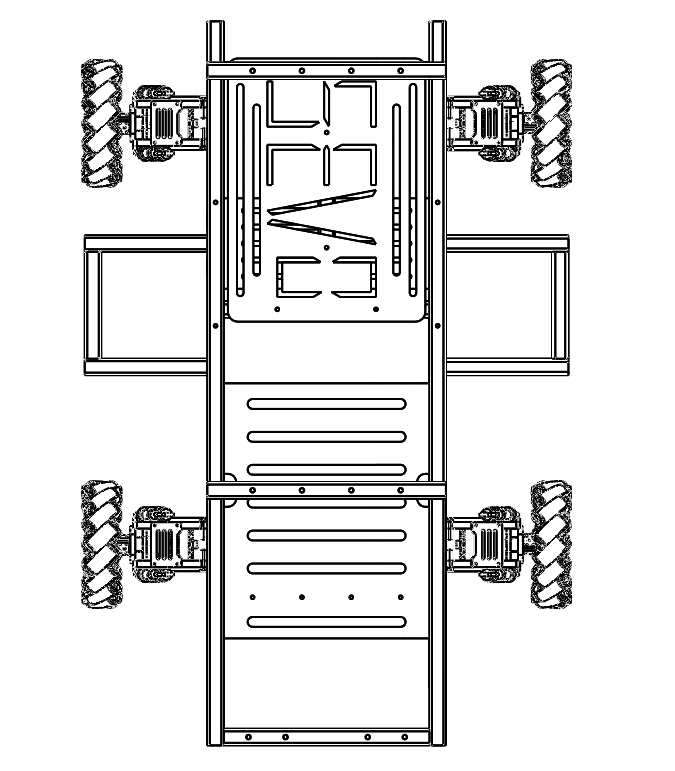
\includegraphics[width=.3\textwidth]{chassis.png}}
  \subcaptionbox{主视图\label{fig:chassis2}}
  {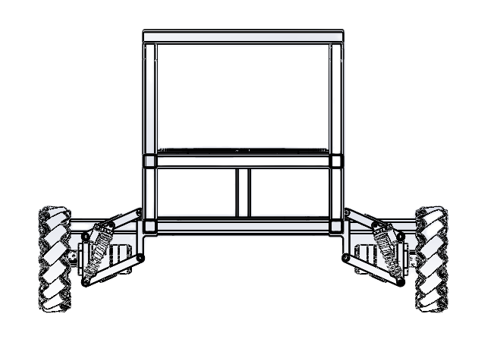
\includegraphics[width=.3\textwidth]{chassis_1.png}}
  \subcaptionbox{侧视图\label{fig:chassis3}}
  {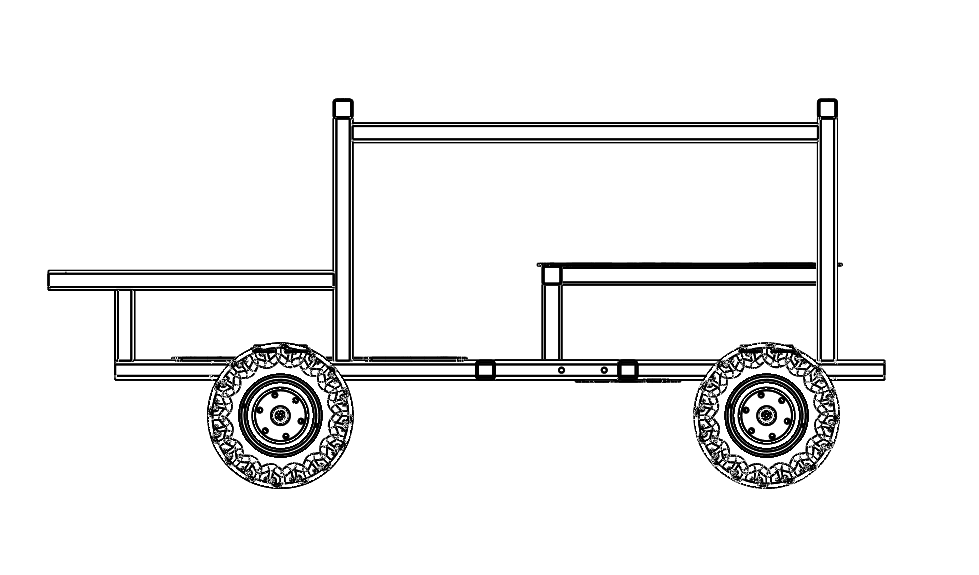
\includegraphics[width=.3\textwidth]{chassis_2.png}}
  \caption{动力模块设计图}
  \label{fig:chassis}
\end{figure}


\begin{figure}
  \centering
  \subcaptionbox{直流无刷减速电机\label{fig:3508}}
  {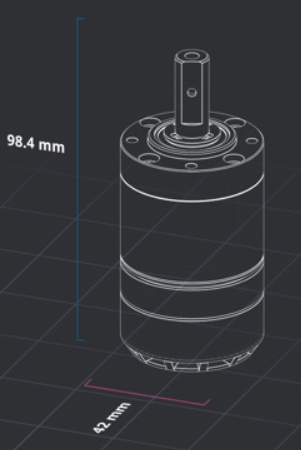
\includegraphics{m3508.png}}
  \subcaptionbox{电子调速器\label{fig:620}}
  {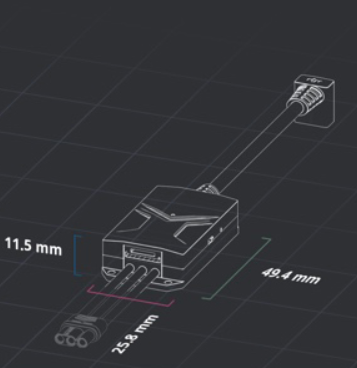
\includegraphics{C620.png}}
  \caption{电机与电子调速器设计图}\label{ele}
\end{figure}

\begin{figure}[htbp]
  \centering
  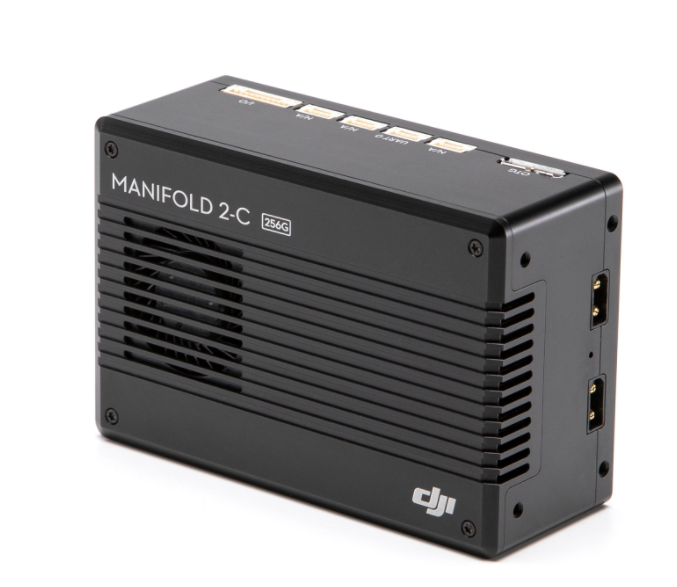
\includegraphics[width=\textwidth]{manifold.png}
  \caption{计算模块}
  \label{fig:manifold}
\end{figure}

\begin{enumerate}[label=\arabic*).]
  \item \textit{动力模块}\\
      动力模块是承载和安装机器人动力系统及其附属部件的机构。如图\ref{fig:chassis}所示使用麦克纳姆轮,支持全向运动。动力系统由RoboMaster M3508 P19 无刷直流减速电机(图\ref{fig:3508})和RoboMaster C620 电子调速器组成(图\ref{fig:620})。
      C620无刷电机调速器采用32位定制电机驱动芯片,配合磁场定向控制(FOC)技术,实现对电机转矩的精确控制。M3508直流无刷减速电机是专为中小型移动平台和机器人等量身打造的高性能伺服电机,可搭配C620电调实现正弦驱动,相比传统方波驱动具有更高的效率、机动性和稳定性。本产品减速箱减速比约为19:1。
  \item \textit{感知模块}\\
      感知模块应组装一个远距高分辨级联模组mmWave-CAS EVM如图\ref{fig:CAS}和四个mmWave EVM如图\ref{fig:mini}所示。根据EVM的版本,安装可能会略有不同。
      在所示示例中,用于安装mmWave EVM的支架是3D打印的。
      对于本演示而言,至关重要的是,必须每隔90度将mmWave EVM安装在机器人周围,与机器人中心等距。
      在所示示例中,将12V至5V转换器安装在顶板中心下方,而USB分配器则放置在顶板下方。四个EVM使用USB分配器连接到计算模块。
  \item \textit{控制模块}\\
      控制模块使用RoboMaster 开发板C型 (STM32F427) 作为主控板,开发板主控芯片为STM32F427IIH6,拥有丰富的扩展接口和通信接口包括12V/5v/3.3v电源接口,CAN接口,UART接口、可变PWM接口、SWD接口,
      板载IMU传感器,可配合RoboMaster出品的M3508、 M2006直流无刷减速电机、UWB模块以及计算模块等产品使用,亦可配合DJI飞控SDK使用,配件丰富。
  \item \textit{计算模块}\\
  计算模块使用的是英特尔酷睿 i7-8550U 处理器,功率范围5-60W,具备优秀的处理能力和响应速度的同时仅有200g左右的超轻重量。
  计算模块详细参数见表\ref{tab:manifold}。
\end{enumerate}


\begin{figure}
  \centering
  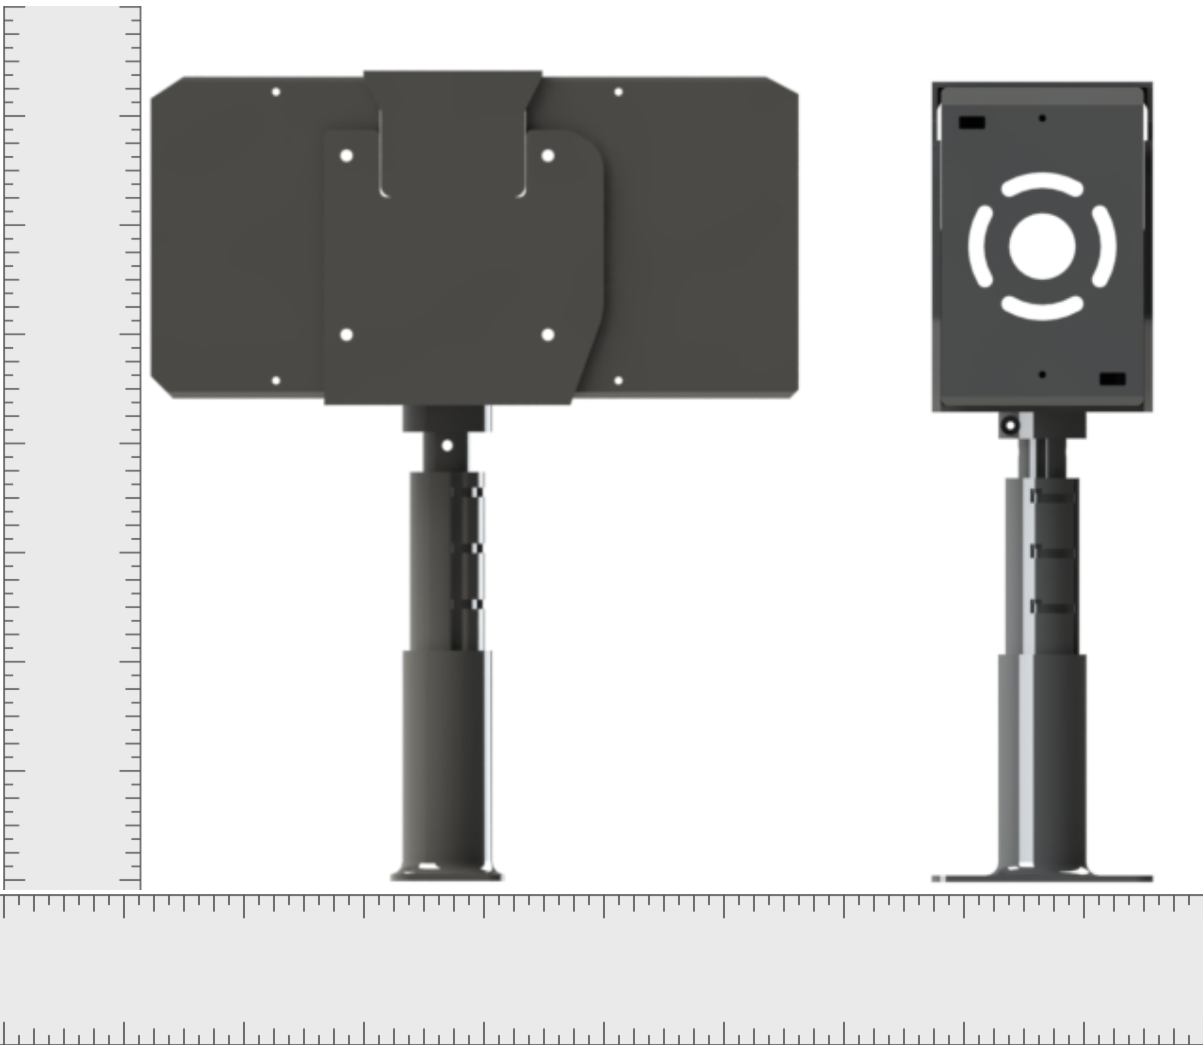
\includegraphics[width=\textwidth]{radar_b.png}
  \caption{mmWave-CAS EVM}\label{fig:CAS}
\end{figure}

\begin{figure}
  \centering
  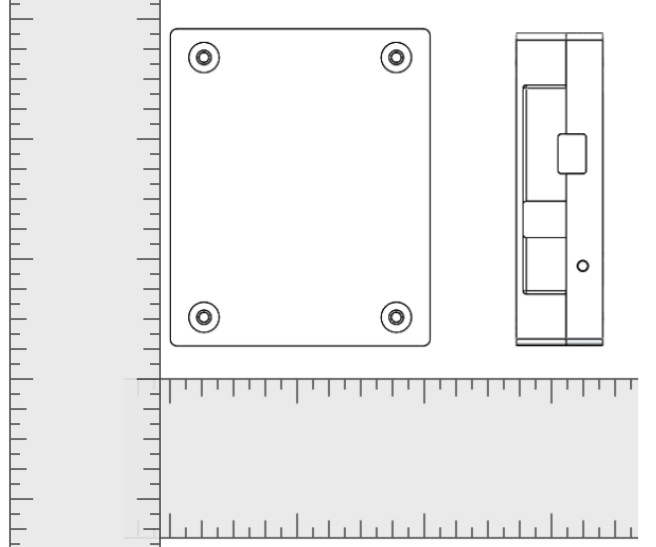
\includegraphics[width=.5\textwidth]{radar_mb.png}
  \caption{mmWave EVM}\label{fig:mini}
\end{figure}
  

\begin{table}[!htbp]
  \centering
  \caption{计算模块规格参数}\label{tab:manifold}
  \begin{tabular}{cc}
    \toprule
    参数名称  & 参考数值  \\
    \midrule
    重量  & 205g   \\
    尺寸 & $91 \times 61 \times 35$ mm  \\
    处理器 &  i7-8550U \\
    内存 & 8GB 64bit,DDR4 2400MHz \\
    SATA-SSD & 256GB\\
    网络 & 千兆以太RJ-45接口\\
    USB & USB3.0(Type A)$\times 2$,USB3.0(Micro-B)$\times 1$ \\
    I/O & UART $\times 1$  \\
    功率 & 5-60w \\
    电源 & 15.2-27.0V电源接口$\times 2$  \\
    工作温度 & -25至45$^{\circ}$C\\
  \bottomrule
  \end{tabular}%
\end{table}%

\subsubsection{软件平台}

软件平台以机器人传感器$\rightarrow$感知$\rightarrow$决策$\rightarrow$规划$\rightarrow$控制$\rightarrow$执行器 的环路进行架构,不同模块具体以ROS Package的形式维护,模块和其数据流如下图所示。
\begin{figure}
  \centering
  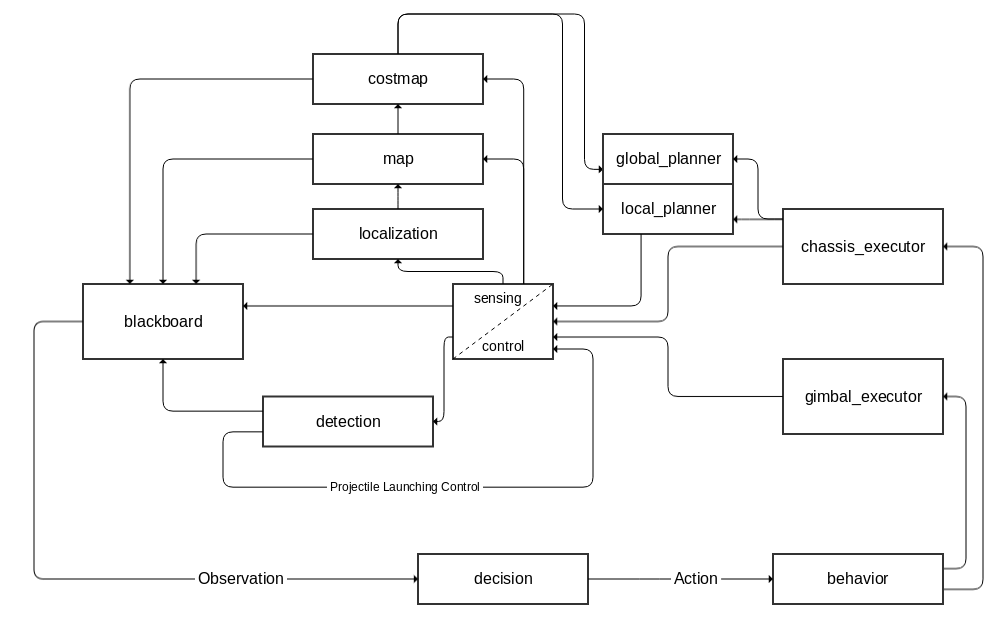
\includegraphics[width=\textwidth]{flow.png}
  \caption{架构与模块介绍}\label{fig:flow}
\end{figure}

\begin{enumerate}[label=\arabic*).]
  \item \textit{传感器、控制器与执行器}\\
      中心模块集成传感器模块(雷达、相机、IMU等)、嵌入式控制平台(执行实时任务,如闭环控制和数据采集与预处理)与执行器(电机等),负责sensing和control两大任务,具体ROS Package为包含嵌入式SDK的roborts\_base,相机的roborts\_camera以及相关传感器驱动包。
  \item \textit{感知部分}\\
      感知部分包括机器人定位、地图的维护和抽象、目标识别与追踪等。localization模块负责机器人定位,是导航系统中强依赖的节点,其主要通过获得一系列的传感器信息,通过特定算法的处理,最终得到机器人坐标系到地图坐标系的变换关系,也就是机器人在地图中的位姿。
      map模块负责机器人地图维护,目前采用ROS开源Package map\_server。
      costmap模块负责代价地图维护,集成了静态地图层,障碍物层和膨胀层,主要用于运动规划部分,不单纯针对规划使用。
      detection模块负责目标识别和追踪,主要利用mmWave-CAS EVM对拍摄到的点云信息进行物体的聚类与跟踪。
  \item \textit{任务调度与决策部分}\\
  任务调度与决策部分包括调度感知输入模块和调度规划执行输出模块的接口,以及决策的核心框架。
  decision模块为机器人决策框架,以行为树(BehaviorTree)为决策框架。blackboard模块调度各种模块的感知任务获取信息,behavior模块集成了离散动作空间的各种动作或行为。
  executor模块是behavior模块的依赖,其包含底盘和云台内不同模块内不同抽象程度的机器人任务委托接口(例如调度底盘运动规划执行)。
  \item \textit{运动规划部分}\\
  运动规划部分是运动规划功能模块,由决策部分中chassis\_executor模块来调度完成导航。global\_planner模块负责机器人的全局路径规划,全局路径规划(简称全局规划)是导航系统中运动规划的第一个步骤,在给定目标位置后,根据感知的全局代价地图搜索得到一条无碰撞的最短路径(即一系列离散的坐标点),然后作为输入传递给局部轨迹规划模块控制机器人的具体运动。全局路径规划A Star算法,
  是一种静态路网中求解最短路最有效的方法。公式表示为:
  $$
    f(n)=g(n)+h(n)
    \label{a*}
  $$
  其中$f(n)$是节点$n$从初始点到目标点的估价函数,$g(n)$是在状态空间中从初始节点到$n$节点的实际代价,$h(n)$是从$n$到目标节点最佳路径的估计代价。在实际的全局路径规划中,静态网路由全局代价地图提供。
  local\_planner模块负责机器人的局部轨迹规划模块,局部路径规划模块根据机器人的里程计信息,雷达的感知信息,结合全局路径规划给出的最优路径,计算出机器人当前能够避免与障碍物碰撞的最优速度。局部路径规划的相关算法参考 Time Elastic Band,算法建立了轨迹执行时间的目标方程,在满足与障碍物保持安全距离, 运动时遵守动力学约束的前提下,优化机器人实际运行轨迹,最终求出机器人可执行的速度。
\end{enumerate}



\subsection{测试方案}
在重量和尺寸检测方面,分别称量设备的重量和尺寸。在功耗测量方面,通过稳压限流模块精准控制单一设备功耗。在建图精度测试方面,通过定位时间戳与室内定位基站作为参考,比较测量误差。
在定位精度方面,在图\ref{fig:map}场地进行测试,通过小车车载LPS定位装置与UWB定位装置,完成规定路径的行驶,通过比较UWB与LPS的定位航迹,计算LPS的定位误差。

\subsection{条件与限制}
本次实验等比例模拟了某区域的城市环境、地面材料及战车尺寸、质量等参数,力图复现一个真实且残酷的战场环境。
但仍受以下客观条件限制。
\begin{enumerate}
  \item  本实验在室内封闭进行,因而无法使用无人机设备进行空中拍摄,故仅提供侧轴视角和POV视角测试视频;
  \item  因为UWB、LPS、IMU和里程计都存在误差,因此定位与建图结果在此误差基础上会存在一定且无法消除的偏移;
  \item  高分辨识别雷达(图\ref{fig:CAS})和建图与导航雷达(图\ref{fig:mini})采用解耦合设计,高分辨识别雷达仅作目标识别之用不参与建图与导航过程;
\end{enumerate}

\section{测试计划}

\subsection{测试项目}
完成设备重量检测、功耗测量、建图精度测试、定位精度测试等内容,为后续实验提供指标参数与参考依据。
测试目标包括高分辨雷达,建图雷达,导航基准为UWB接收机。

\subsection{测试技术流程}

\subsubsection{硬件指标测量}
直接对设备测量即可。测量项目包括尺寸,质量,设备功耗等。

\subsubsection{软件指标测试}
首先连接STM32设备的虚拟串口,lsusb可以查看Vendor和Product的ID,然后创建并配置/etc/udev/rules.d/roborts.rules文件:
\begin{lstlisting}[language=bash]
  KERNEL=="ttyACM*", ATTRS{idVendor}=="0483", ATTRS{idProduct}=="5740", 
  MODE:="0777", SYMLINK+="serial_sdk"
\end{lstlisting}
同理配置雷达。然后重新加载并启动udev服务,可能需要重新插拔设备后生效。
\begin{lstlisting}[language=bash]
  SUBSYSTEM=="tty", ATTRS{idVendor}=="10c4", ATTRS{idProduct}=="ea70",
  SYMLINK+="mmWave_%s{serial}_%E{ID_USB_INTERFACE_NUM}"
\end{lstlisting}
将北向传感器插入远程笔记本电脑,然后在命令行中键入以下内容:
\begin{lstlisting}[language=bash]
  ls -l /dev/ | grep mmWave
\end{lstlisting}
应出现两个符号链接,一个对应命令端口,一个对应数据端口。
重复步骤,插入每个传感器,并在相应的方向启动文件中更改command\_port和data\_port字段。
配置多个相同型号的雷达的会麻烦一些,由于Vendor和Product的ID是一样的,因此要查看每个数据端口具体的特性。
\begin{lstlisting}[language=bash]
  udevadm info --attribute-walk --name=/dev/ttyACM*
\end{lstlisting}

\subsubsection{环境感知指标测量}

\begin{figure}[htbp]
  \centering
  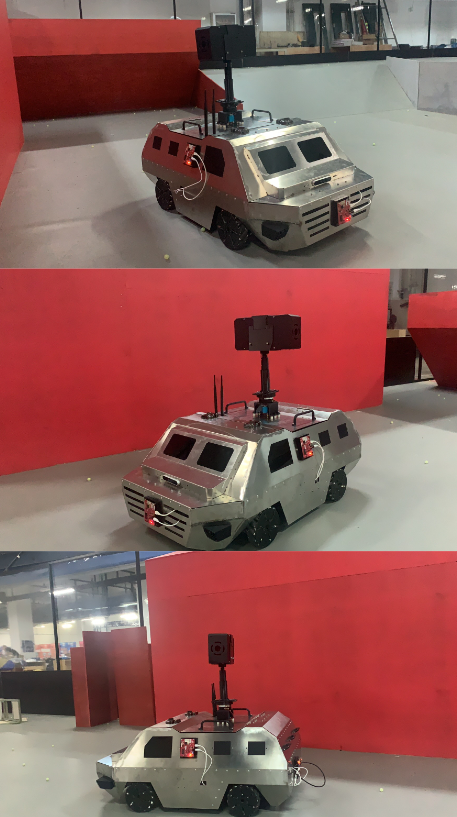
\includegraphics[width=.5\textwidth]{up.png}
  \caption{整车装配图}
  \label{fig:car}
\end{figure}

\begin{figure}[htbp]
  \centering
  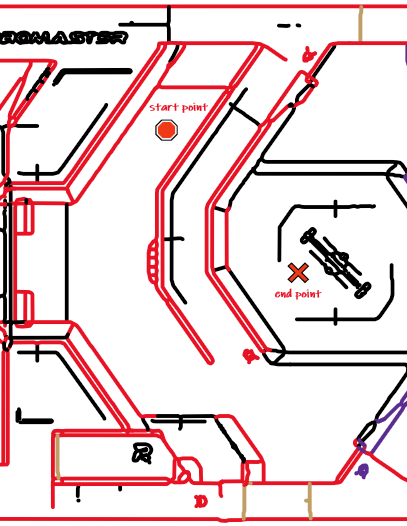
\includegraphics[width=.5\textwidth]{octmap.png}
  \caption{实验场配置草图}
  \label{fig:octmap}
\end{figure}

首先如图\ref{fig:car}中所示,装配整车四片导航雷达和前置摄像头,并如图\ref{fig:octmap}所示,将战车放置在图中起点位置。
并在图所示场地中红线位置设置障碍物。红点位置设置LPS基站,并与战车定位系统同步。将定位值输入电脑中;
启动远程控制程序:
\begin{lstlisting}[language=ros]
  roslaunch mmwave_launchers my_teleop.launch
\end{lstlisting}
打开一个新的终端窗口,将ssh连接到计算模块并运行以下命令打开所有雷达:
\begin{lstlisting}[language=ros]
  roslaunch mmwave_launchers sensor_bringup.launch
  roslaunch mmwave_launchers sensor_left.launch
  roslaunch mmwave_launchers sensor_right.launch
  roslaunch mmwave_launchers sensor_back.launch
\end{lstlisting}
聚焦远程控制窗口,遥控战车完成建图。

\subsubsection{自主导航指标测量}

\begin{figure}[htbp]
  \centering
  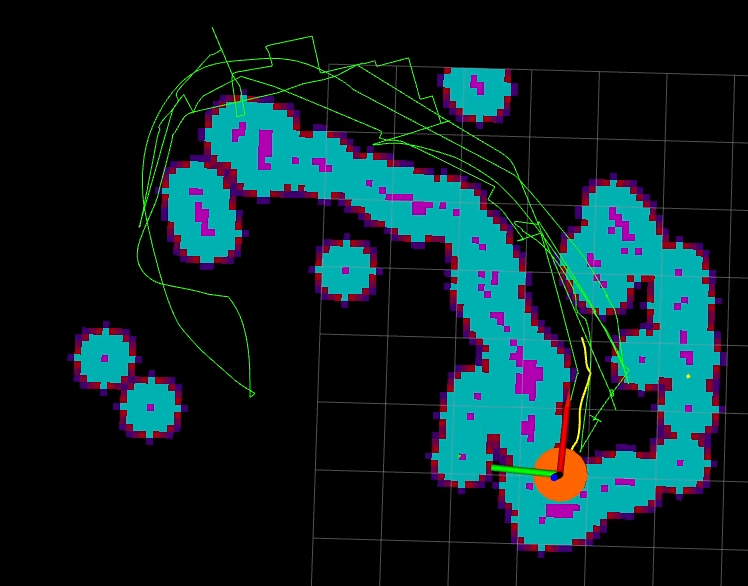
\includegraphics[width=\textwidth]{getmap.png}
  \caption{雷达建立地图}
  \label{fig:getmap}
\end{figure}
\begin{figure}[htbp]
  \centering
  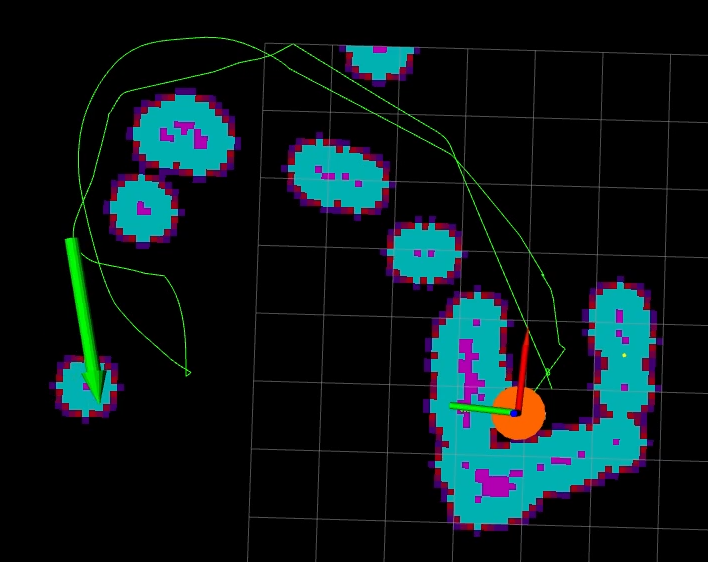
\includegraphics[width=\textwidth]{navgoal.png}
  \caption{提供导航目标}
  \label{fig:goal}
\end{figure}


首先如图\ref{fig:getmap}中所示,获取环境感知实验得到的雷达建图结果。
\begin{lstlisting}[language=ros]
  rosrun octomap_server octomap_server_node <pathtomap>.bt
\end{lstlisting}	
打开导航程序。
\begin{lstlisting}[language=ros]
  roslaunch mmwave_launchers crl_navigation.launch
  rosrun my_plugin smooth_vel
\end{lstlisting}
为导航栈提供初始姿态估计,开始导航。选择2D Pose Estimate(沿屏幕顶部),
然后单击战车在地图中的位置,并沿其面对的方向拖动。看到战车出现在起点时,点击后立即释放。
再通过选择2D Nav goal并单击导航目标到位置并沿其面对的方向拖动,(如图\ref{fig:goal}所示)
为战车指定一个导航目标。释放安全遥控后,应该开始导航到它的目标。

\section{测试结果}
\subsection{重量检测}
\begin{figure}[htbp]
  \centering
  \includegraphics[width=\textwidth]{m.jpg}
  \caption{高分辨雷达质量测量}
  \label{fig:m}
\end{figure}
\begin{figure}[htbp]
  \centering
  \includegraphics[width=\textwidth]{m2.jpg}
  \caption{环境感知雷达质量测量}
  \label{fig:m2}
\end{figure}
通过对雷达与设备称重,如图\ref{fig:m}高分辨所示,高分辨雷达重量1.170kg,达到指标要求。
如图\ref{fig:m2}所示,环境感知雷达重量0.1kg,达到指标要求。

\subsection{尺寸检测}
\begin{figure}[htbp]
  \centering
  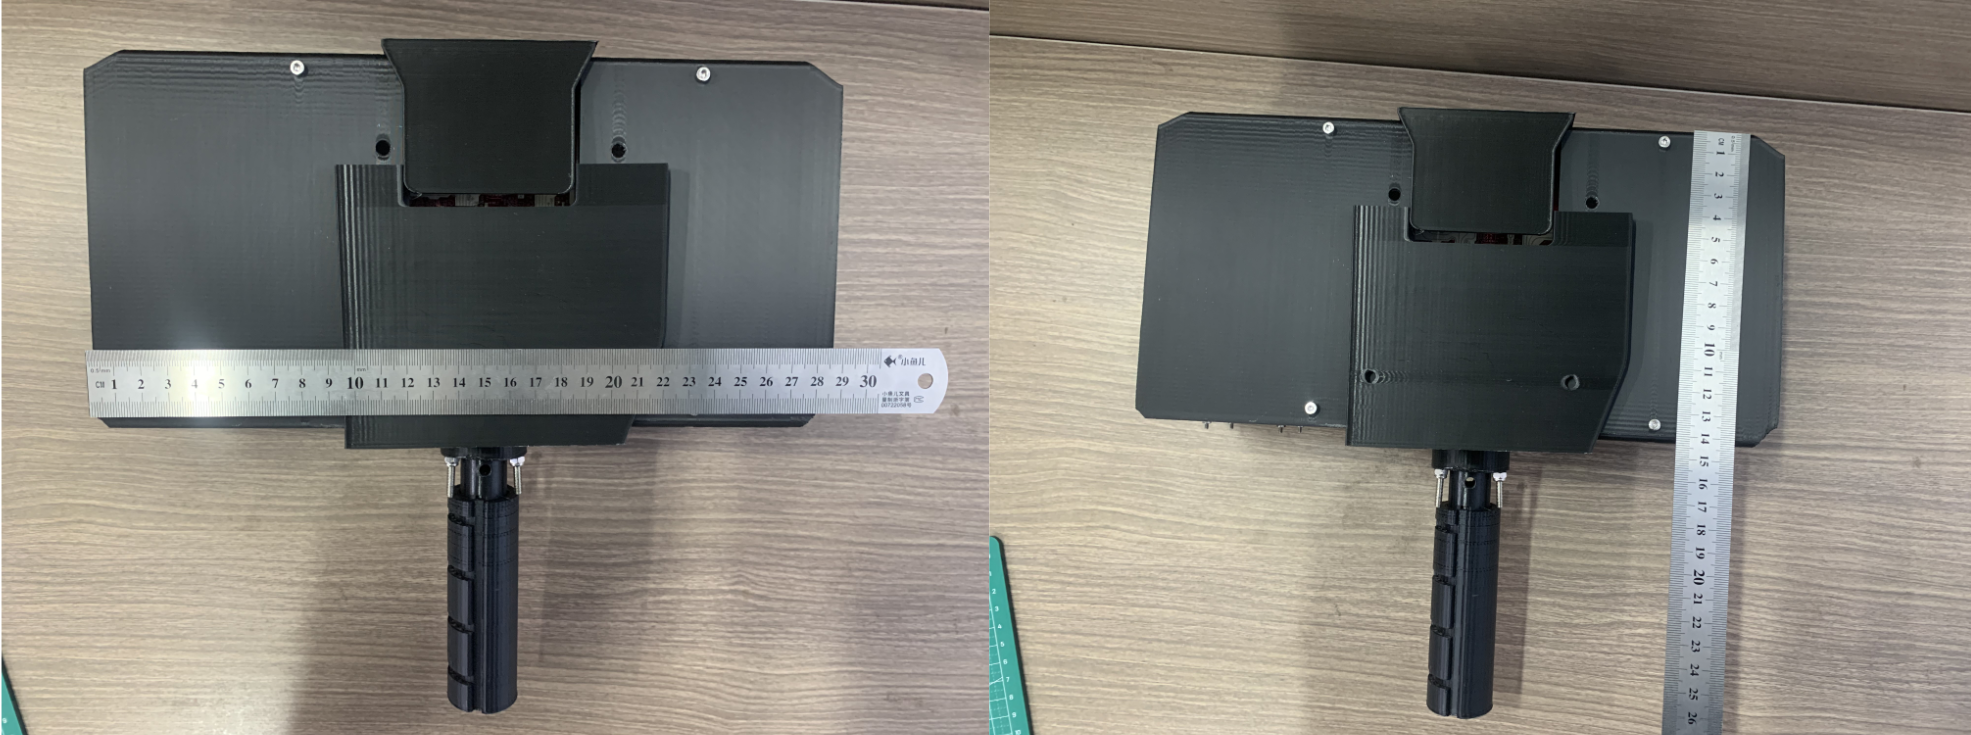
\includegraphics[width=\textwidth]{s1.png}
  \caption{高分辨雷达尺寸测量}
  \label{fig:s1}
\end{figure}
\begin{figure}[htbp]
  \centering
  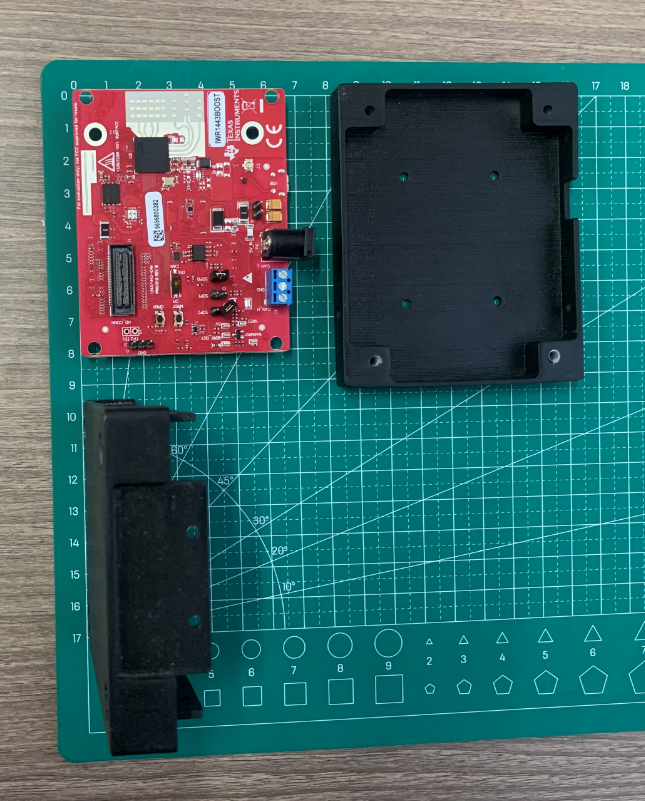
\includegraphics[width=.5\textwidth]{s2.png}
  \caption{环境感知雷达尺寸测量}
  \label{fig:s2}
\end{figure}

通过对雷达与设备尺寸测量,如图\ref{fig:s1}所示,高分辨雷达体积$97mm \times 285mm \times 143mm$,达到指标要求。
如图\ref{fig:s2}所示,环境感知雷达体积$15mm \times 70mm \times 80mm$,达到指标要求。

\subsection{功率检测}
通过对环境感知雷达利用稳压限流模块驱动,如图所示,工作功率2.5W,达到指标要求。

\subsection{环境感知检测}
\begin{figure}[htbp]
  \centering
  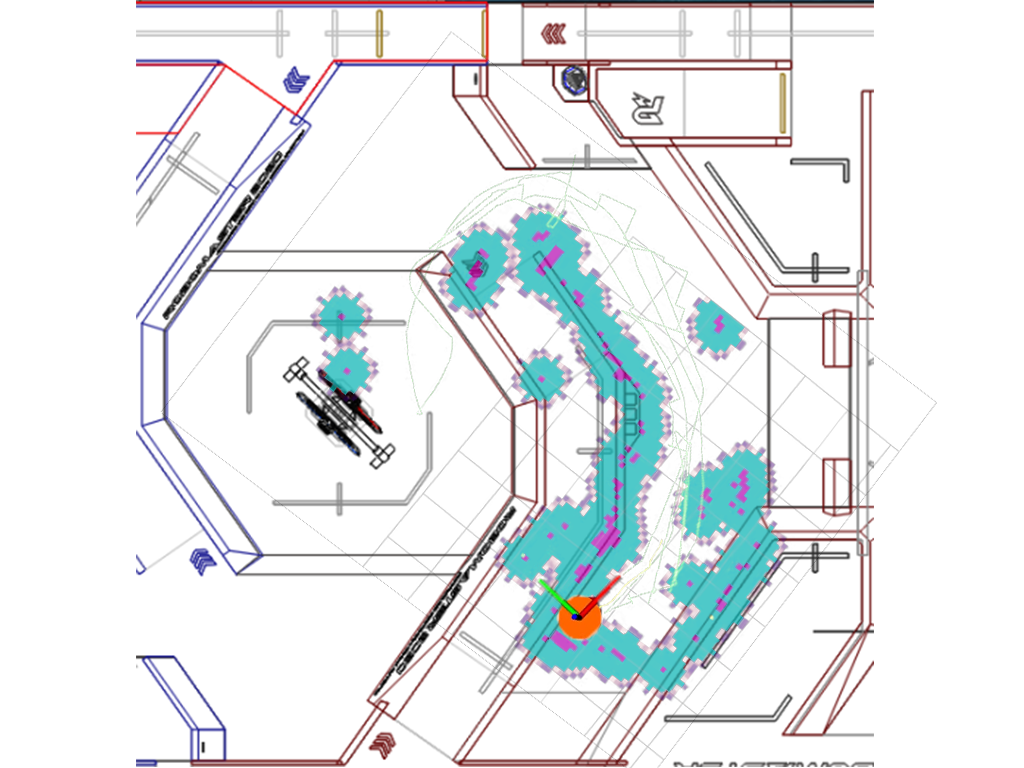
\includegraphics[width=\textwidth]{maptest.png}
  \caption{环境感知检测结果}
  \label{fig:maptest}
\end{figure}
通过对在建图结束时刻与结束时所保存的地图文件与场地设计文件以及LPS基站和车载里程计信息交叉比对,
并取对误差取绝对值,求得同时定位与建图误差;通过实验,其测距误差如图\ref{fig:maptest}所示,误差在1mm到10mm之间,
达到指标要求的10mm以内。

\subsection{自主导航检测}

\begin{figure}[htbp]
  \centering
  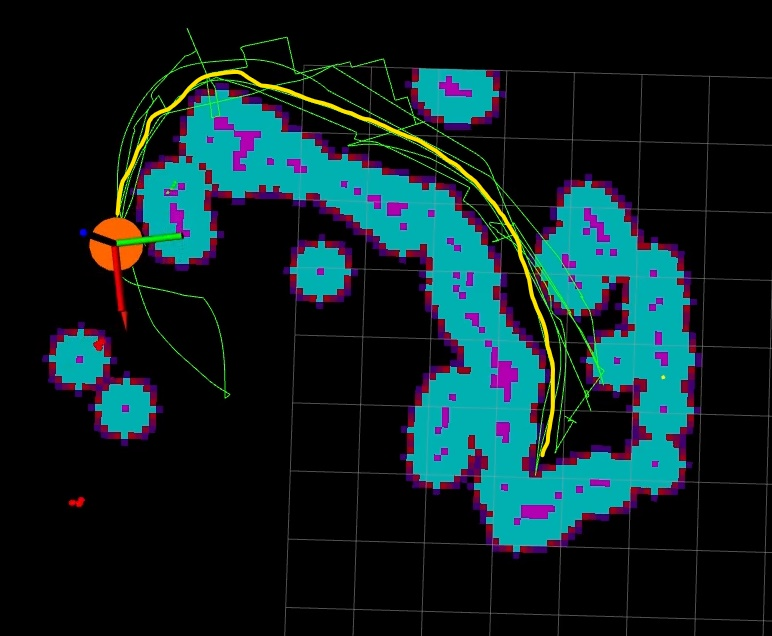
\includegraphics[width=\textwidth]{finish.jpg}
  \caption{自主导航检测结果}
  \label{fig:navtest}
\end{figure}

图\ref{fig:car}为实验战车,车上包括环境感知设备与LPS设备,场地见图\ref{fig:map}。
按照图\ref{fig:goal}配置车辆后释放战车。战车再运行过程中,黄色线条为实时规划路径。图\ref{fig:navtest}可以看出战车
在环境感知设备的辅助下无碰撞的完成了避障自主导航。


\bibliography{wpref}

\end{document}
